\section{COPS}
\begin{frame}
\frametitle{COPS}
\begin{block}{Cos'è COPS}
COPS (Cluster of Order-Preserving Servers) è, come Dynamo,
un key-value store distribuito in un'ampia area che implementa un modello di coerenza
denomitato \textit{causal+}.
\end{block}
%L'approccio principale su cui si basa COPS consiste nel tracciare e controllare esplicitamente
%le dipendenze causali fra le chiavi nel cluster locale prima di esporre una qualunque scrittura.
\begin{block}{Cos'è COPS-GT}
COPS-GT è un'evoluzione di COPS che implementa le cosiddette le \texttt{get transaction},
capaci di ottenere una visione consistente di un insieme di chiavi.
\end{block}
\end{frame}

\begin{frame}
\frametitle{Obiettivi di COPS}
	\begin{definizione}
	Un \alert{sistema ALPS} è un sistema caratterizzato da 4 proprietà:
	\begin{enumerate}
		\item<1-> Availability \\
				  Ogni richiesta riceve una risposta su ciò che è riuscito o fallito.
		\item<1-> Low Latency \\
				  Le operazioni completano velocemente.
		\item<1-> Partition-tolerance \\
				  Il sistema continua a funzionare nonostante arbitrarie perdite di messaggi:
				  in questi casi alcuni nodi possono rimanere isolati dagli altri e non avere
				  più informazioni aggiornate (sono partizionati).
		\item<1-> High Scalability \\
				  Possiamo aumentare la capacità del sistema.
	\end{enumerate}
	\end{definizione}
\end{frame}

\begin{frame}
\frametitle{Architettura del sistema}
	\begin{figure}
		\centering
		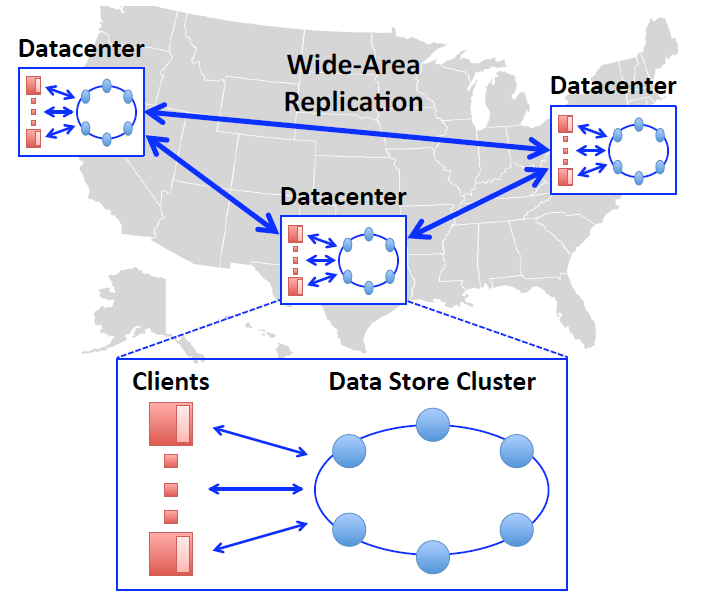
\includegraphics[scale=0.45]{COPS/COPS1.png}
	\end{figure}
\end{frame}

\begin{frame}
\frametitle{Potenziale di causalità}
	\begin{definizione}
	Definiamo il \alert{potenziale di causalità} fra operazioni (e lo denotiamo con 
	il simbolo $\rightsquigarrow$) come una relazione che soddisfa le seguenti tre regole:
	\begin{enumerate}
		\item<1-> \textbf{Execution thread.}
				  Se $a$ e $b$ sono due operazioni in un singolo thread di esecuzione
				  allora $a \rightsquigarrow b$ se l'operazione $a$ accade prima dell'operazione $b$;
		\item<1-> \textbf{Gets From.}
				  Se $a$ è un'operazione di \texttt{put} e $b$ è un'operazione di
				  \texttt{get} che ritorna il valore scritto da $a$, allora $a \rightsquigarrow b$;
		\item<1-> \textbf{Transitivity.}
				  Date tre operazioni $a$, $b$, $c$, se $a \rightsquigarrow b$ e $b 
				  \rightsquigarrow c$, allora $a \rightsquigarrow c$.
	\end{enumerate}
	\end{definizione}
\end{frame}

\begin{frame}
\frametitle{Un esempio}
	\begin{figure}
		\centering
		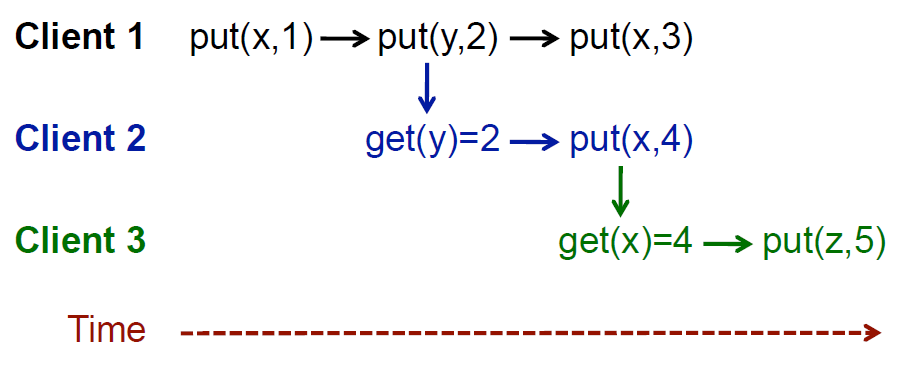
\includegraphics[scale=0.40]{COPS/COPS2.png}
	\end{figure}
\end{frame}

\begin{frame}
\frametitle{Casual+ Consistency}
\begin{definizione}
Definiamo la \alert{Causal+ Consistency} implementata da COPS come una combinazione di due proprietà:
	\begin{itemize}
		\item<1-> Causal Consistency \\
				  I valori restituiti da un'operazione di \texttt{get} da una replica sono 
				  consistenti con l'ordine definito da $\rightsquigarrow$;
		\item<1-> Convergent conflict handling \\
				  Tutte le operazioni di \texttt{put} in conflitto vengono gestite nello
				  stesso modo da tutte le repliche, usando una funzione di gestione $h$ (associativa
				  e commutativa).
	\end{itemize}
\end{definizione}

\begin{definizione}
Si dice che due operazioni $a$ e $b$ sono \alert{in conflitto} se sono entrambe
due operazione di \texttt{put} ``simultanee'' sulla stessa chiave.
\end{definizione}
\end{frame}
% I conflitti sono indesiderabili per due ragioni:
% 	1) Non sono ordinabili dalla causal consistency!
%	2) Permettono a due o più repliche di divergere per sempre!

\begin{frame}
\frametitle{Coerenze a confronto}
\begin{block}{Sequential consistency}
Il risultato di qualunque operazione è uguale a quello ottenuto se le operazioni
di read e di write da parte di tutti i processi sullo archivio di dati fossero eseguite:
	\begin{enumerate}
		\item in un qualche ordine sequenziale;
		\item le operazioni di ogni singolo processo appaiono comunque in questa sequenza
			  nell'ordine specificato dal programma.
	\end{enumerate}
\end{block}	
	\begin{figure}
		\centering
		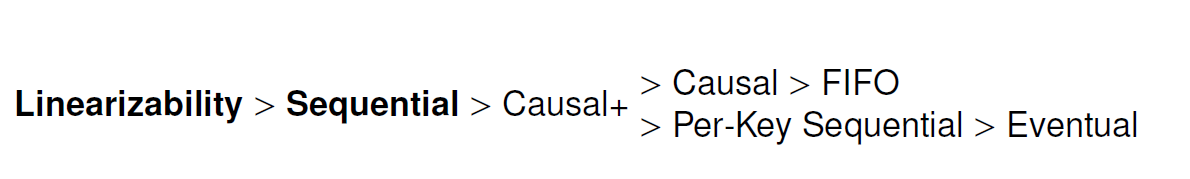
\includegraphics[scale=0.35]{COPS/COPS6.png}
	\end{figure}

Se in Dynamo abbiamo un livello di coerenza che può oscillare fra Strong ed Eventual,
in COPS la definizione risulta più netta: si cerca di implementare il meglio che si può
avere con le caratteristiche ALPS!
\end{frame}

\begin{frame}
\frametitle{Astrazioni di COPS (I)}
\begin{block}{Versione}
Ci riferiamo a differenti valori di una data chiave come alla loro \alert{versione}
(e la indichiamo con $\text{key}_{version}$).
\end{block}
Una volta che una data replica in COPS ritorna un certo valore di una data chiave,
siamo assicurati, per casual+ consistency, che i successivi valori richiesti a quella
replica di quella data chiave saranno quello ottenuto o una sua versione successiva,
mai precedente.\\
\textit{(PROPRIETA' DI PROGRESSIONE)}
\end{frame}

\begin{frame}
\frametitle{Astrazioni di COPS (II)}
\begin{block}{Dipendenze}
Diciamo che $y_i$ \alert{dipende da} $x_i$ se e solo se \texttt{put}$(x_i)
\rightsquigarrow$ \texttt{put}$(y_i)$.
\end{block}
Tutte le operazioni che causalmente precedono una data operazione devono aver effetto
prima che quella operazione avvenga.
\end{frame}

\begin{frame}
\frametitle{Design di COPS (I)}
\begin{block}{Struttura di COPS}
COPS è formato da due componenti principali:
\begin{itemize}
	\item<1-> Key-value store \\
			  Coppie <key, value> alle quali sono associati metadati (numero di versione
			  e lista di dipendenze).
	\item<1-> Client library \\
			  Esporta due operazioni principali alle applicazioni: letture via \textit{get}
			  e scritture via \textit{put}.
\end{itemize}
\end{block}
\end{frame}
% Ogni coppia key-value ha associati dei matadati: in COPS questi metadati sono il numero
% di versione, mentre in COPS-GT sono il numero di versione e una lista delle dipendenze
% (ossia una lista di chiavi con la corrispondente versione da cui si dipende)

\begin{frame}
\frametitle{Design di COPS (II)}
L'interfaccia di COPS è composta da quattro operazioni (più una):
\begin{itemize}
	\item<1-> \textit{ctx\char`_id} $\leftarrow$ \texttt{createContext()}
	\item<1-> \textit{bool} $\leftarrow$ \texttt{deleteContext}\textit{(ctx\char`_id)}
	\item<1-> \textit{bool} $\leftarrow$ \texttt{put}\textit{(key, value, ctx\char`_id)}
	\item<1-> \textit{value} $\leftarrow$ \texttt{get}\textit{(key, ctx\char`_id)}
	\item<1-> \textit{values} $\leftarrow$ \texttt{get\char`_trans}\textit{(keys, ctx\char`_id)}
\end{itemize}
\begin{figure}
	\centering
	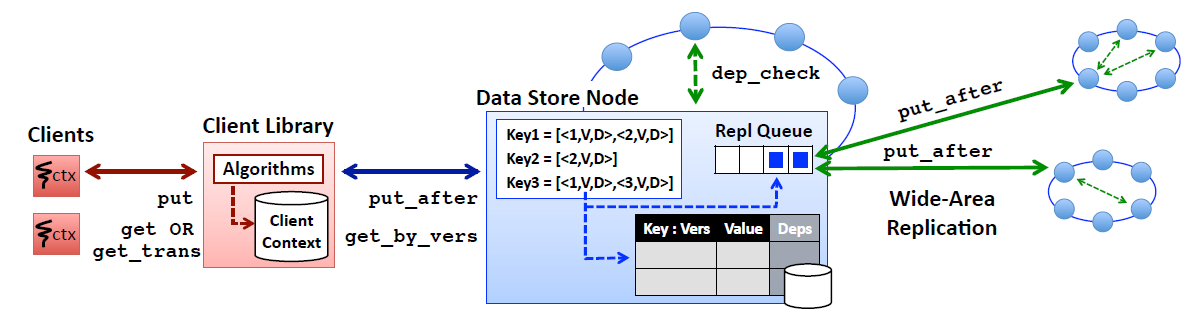
\includegraphics[scale=0.35]{COPS/COPS7.png}
\end{figure}
%\begin{figure}
%	\centering
%	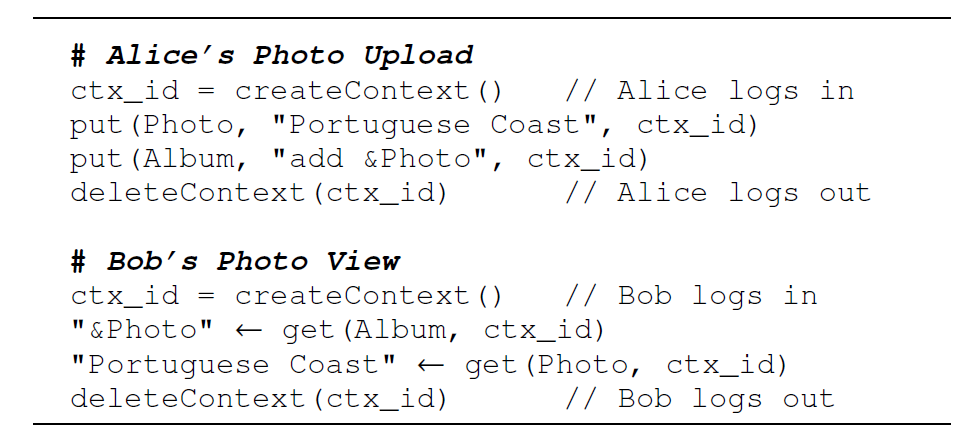
\includegraphics[scale=0.35]{COPS/COPS3.png}
%\end{figure}
\end{frame}
% Il contesto mi permette di separare e riconoscere i diversi thread di esecuzione
% Il contesto contiene anche le dipendenze fra le variabili

\begin{frame}
\frametitle{Dipendenze}
%COPS codifica le dipendenze all'interno di metadati associati ad ogni versione
%di una chiave. Di seguito presentiamo un esempio nel dettaglio:
Il contesto viene usato internamente da COPS per tenere traccia delle dipendenze causali
che si vengono a generare quando sono eseguite di volta in volta operazioni di \texttt{put}
e di \texttt{get} da parte dei client. \\
Quella che si viene a creare è quindi una rete di dipendenze come mostrato di seguito:
\begin{figure}
	\centering
	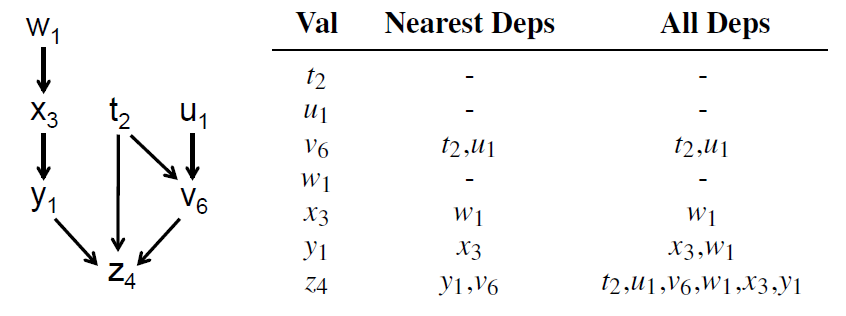
\includegraphics[scale=0.35]{COPS/COPS4.png}
\end{figure}
La proliferazione di metadati riduce l'efficienza: possiamo affidarci
alle ``nearest dependencies''!
\end{frame}

\begin{frame}
\frametitle{Scritture}
Tutte le scritture in COPS:
\begin{enumerate}
	\item Vengono eseguite sul cluster locale;
	\item Vengono propagate in maniera asincrona sui cluster remoti.
\end{enumerate}
Il sistema fornisce due API per gestire questo processo:
\begin{itemize}
	\item \texttt{put\char`_after} \\
		  Consente di eseguire entrambe le operazioni di \emph{write} in un 
		  colpo solo e ci assicura che il valore è committato ad ogni cluster solo dopo che tutte
		  le sue dipendenze sono state scritte (su quello specifico cluster).
	\item \texttt{dep\char`_check} \\
		  Verifica che le dipendenze causali siano soddisfatte sul cluster locale, a seguito
		  della ricezione di una \texttt{put\char`_after}.
\end{itemize}
\end{frame}

\begin{frame}
\frametitle{Gestione dei conflitti}
\begin{block}{Conflict handling}
COPS può gestire conflitti in diversi modi a seconda dell'implementazione:
	\begin{itemize}
		\item<1-> Last-writer-win-rule \\
				  (detta Thomas Write rule e basata su Timestamp);
				  % La regola dice che se TS(T) < WTS(O), la corrente azione di scrittura è stata resa 
				  % obsoleta dalla più recente operazione di scrittura di O, che segue la scrittura corrente 
				  % basandosi sull'ordinamento del Timestamp.
		\item<1-> Marking dei conflitti e risoluzione con altri mezzi.
	\end{itemize}
\end{block}
\begin{block}{Lamport Timestamp}
Vengono usati i Lamport Timestamp per assegnare un numero di versione univoco a ogni aggiornamento.
Il nodo setta la parte alta dei bit del numero di versione pari al suo Lamport clock, mentre la
parte bassa viene posta pari all'identificativo univoco del nodo. \\
\end{block}
Non vengono usati i Vector Clock come invece avviene in Amazon Dynamo perché
si ritiene che in un sistema troppo grande potrebbero andare fuori controllo.
\end{frame}

\begin{frame}
\frametitle{Get Transaction}
\begin{block}{Limiti di COPS}
Leggere un insieme di chiavi dipendenti usando una singola operazione di \texttt{get}
non assicura una consistenza causal+, anche se il data store implementa esso stesso
una politica di causal+ consistency.
\end{block}
\begin{block}{Novità di COPS-GT}
COPS-GT offre un'operazione di \texttt{get\char`_trans} che permette di
ritornare una visione consistente di più chiavi.
\end{block}
Questo tipo di transazioni non richiedono locks, sono non bloccanti e
vengono realizzate al più in due rounds.
\end{frame}

\begin{frame}
\frametitle{Pseudocodice}
Presentiamo un esempio di pseudocodice della \texttt{get\char`_trans}:
\begin{figure}
	\centering
	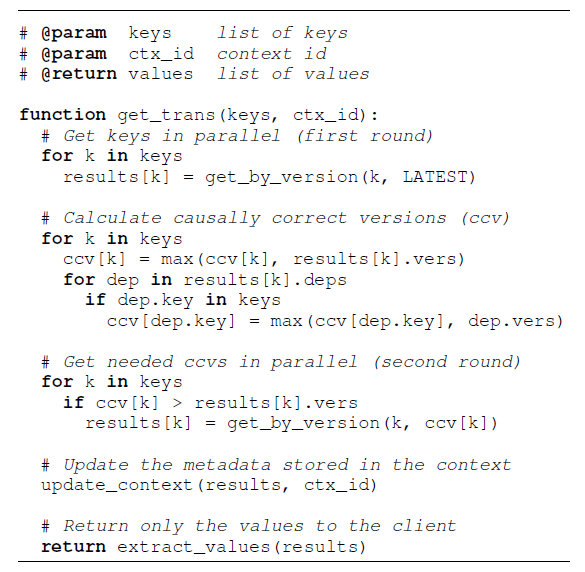
\includegraphics[scale=0.40]{COPS/COPS5.png}
\end{figure}
\end{frame}

\begin{frame}
\frametitle{Concludendo su COPS}
\begin{block}{Vantaggi di COPS}
COPS è un sistema che offre le seguenti caratteristiche:
	\begin{itemize}
		\item<1-> Serve le operazioni localmente, replica in background \\
				  (always on)
		\item<1-> Partiziona lo spazio delle chiavi in più nodi \\
				  (scalabilità)
		\item<1-> Controllo delle repliche con il tracciamento delle dipendenze \\
				  (casual+ consistency)
	\end{itemize}
\end{block}
\begin{block}{Svantaggi}
\end{block}
\end{frame}
